\section{Problem Area}

\subsection{Artificial neural networks}
Computers excel at performing tasks that can be described as a series well-defined steps, and can at these tasks easily outperform humans in doing so.
Tasks that humans find easy, such as understating speech or recognizing faces has proven to be difficult to describe a series of unambiguous operations in the conventional computation model.
Biological neural networks, such as brains, have evolved to be very good at pattern recognition and data classification.
Artificial neural networks(ANN) take inspiration from how biological neural networks process data.

ANN's consist of interconnected processing units(neurons) which work in parallel to solve a specific problem.
The neurons employ a simplified model of how a biological neuron works.
The operation of an artificial neuron consists of two main components, depicted in figure \ref{fig:artificial-neuron}.
 
\begin{figure}[H]

	\centering
	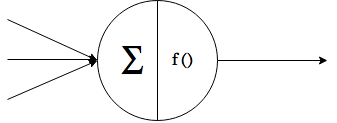
\includegraphics[width=0.5\textwidth]{chapters/res/Neuron.png}
	\caption{Model of an artificial neuron.}
	\label{fig:artificial-neuron}
\end{figure}
First, the neuron sums the action potential from the preceding neurons.
The activation function is then applied on the sum which produces a new action potential as the output.

The connection strength between neurons is simulated by introducing weights on the connections.
A neuron with a higher weight on one of its connections will then be more influenced by that particular connection.
Learning can then be performed by modifying the weights on the connections in the ANN.


The neurons in ANN's are organized into multiple layers, where each neuron is connected to the neurons in the preceding layers.
Typically there is a input layer, an output layer, and zero or more hidden layers between them.

\begin{figure}[H]
	\centering
	\includegraphics[width=0.8\textwidth]{chapters/res/Simple-MLP.png}
	\caption{A feed forward network.}
	\label{fig:mlp-simple}
\end{figure}

Figure \ref{fig:mlp-simple} depicts a simple feed forward network with one hidden layer.
The inputs are propagated from the input layer on the left to the output layer.
More complex network topologies introduce connections within the layers and connections back to preceding layers.

ANN's are used for many applications, including robotics.
Creating good robot controllers can be difficult as the number of sensors and actuators grow.
The designers may know what desired behavior for the robots is, but expressing this in the conventional computing model as a series of instructions can be difficult.
Instead, with machine learning an ANN can learn from examples of desired behavior provided by the controller designers.
This approach allows designers to create the desired controllers by providing examples instead of knowing the exact solution.
